\documentclass{article}

% NeurIPS 2026 style (double-blind workshop review)
\usepackage[dblblindworkshop]{neurips_2026}
\workshoptitle{Who Verifies the Agents? Toward Reliable Agent Development}

% Math and formatting
\usepackage{amsmath,amssymb,amsthm}
\usepackage{booktabs}
\usepackage{graphicx}
\usepackage{xcolor}
\usepackage{hyperref}
\usepackage{caption}
\usepackage{subcaption}
\usepackage{pgfplots}
\usepackage{pgfplotstable}
\usepackage{tikz}
\usepackage{multirow}
\usepackage{array}
\usepackage{colortbl}
\usepackage{enumitem}
\usepackage{wrapfig}
\usepackage{float}
\usepackage{microtype}

\pgfplotsset{compat=1.18}

\tolerance=1000
\hbadness=1000
\emergencystretch=3em

% Custom theorem environments
\newtheorem{finding}{Finding}
\newtheorem{hypothesis}{Hypothesis}

% Color palette
\definecolor{baselineblue}{RGB}{31, 119, 180}
\definecolor{hackableorange}{RGB}{255, 127, 14}
\definecolor{kllowgreen}{RGB}{44, 160, 44}
\definecolor{klmedgreen}{RGB}{0, 100, 0}
\definecolor{klhighgreen}{RGB}{0, 60, 0}
\definecolor{capred}{RGB}{214, 39, 40}
\definecolor{comboguard}{RGB}{148, 103, 189}
\definecolor{lightgray}{RGB}{220, 220, 220}

\title{Do Reward Hacking Guardrails Reduce Exploration Diversity in GRPO?}

\author{Anshul Tripathi \\
  Indian Institute of Technology Roorkee \\
  \texttt{anshul\_t@ee.iitr.ac.in} \\
}

\begin{document}

\maketitle

\begin{abstract}
Reinforcement learning with verifiable rewards, particularly Group Relative Policy Optimization (GRPO), has become a standard approach for training reasoning models. Proxy reward signals, such as length bonuses, create incentives for reward hacking, and practitioners commonly respond with guardrails such as KL regularization or hard length caps, mechanisms that constrain what a policy can earn reward for and so function as a form of verification on the policy's behavior during training. Whether these guardrails change the diversity of a policy's reasoning strategies, and whether that effect is itself reliable across training seeds, has not been systematically measured. We study this question using Qwen2.5-1.5B-Instruct fine-tuned with LoRA on the Countdown arithmetic task, across seven conditions: a clean baseline, a hackable length-bonus reward, three KL-regularized variants at $\beta \in \{0.01, 0.05, 0.10\}$, a hard length cap, and a combined KL-plus-cap guardrail. The six core conditions and the combined condition are each trained with three random seeds; a length-cap severity sweep at four cap values uses a single seed and is reported as preliminary. We measure diversity through pass@k, the pass@k minus pass@1 exploration gap, unique solution count, and the embedding variance of sampled reasoning traces. Our most robust result is that KL regularization increases semantic diversity monotonically with $\beta$ (embedding variance 0.134 to 0.286, exact Jonckheere-Terpstra trend test $p=0.0009$), with a corresponding cost to greedy accuracy. Hard length caps show a qualitatively different and less reliable pattern: two of three seeds internalize the cap and collapse embedding variance to roughly a quarter of baseline, but the third seed fails to internalize the constraint entirely, a bimodal outcome rather than a single guaranteed effect. Embedding variance and unique solution count, our two diversity metrics, are themselves largely uncorrelated across the seven conditions and diverge sharply within the KL series, where embedding variance rises as unique solution count falls; at matched embedding variance, the combined guardrail recovers a markedly higher unique solution count and pass@8 than the high-KL condition alone, without leading the full table on unique solution count. Together these results show that the specific mechanism of a guardrail, not the presence of reward hacking itself, determines whether a trained policy stays exploratory or collapses onto a narrow strategy, that this outcome can depend on the training seed rather than being guaranteed by the guardrail alone, and that which diversity metric is reported can change the apparent verdict on a given guardrail.
\end{abstract}

\section{Introduction}

Reasoning models trained with reinforcement learning from verifiable rewards have advanced rapidly. DeepSeek-R1 \citep{deepseek2024} demonstrated that Group Relative Policy Optimization (GRPO) \citep{shao2024} can train models to produce structured reasoning traces on tasks where correctness is automatically checkable, without relying on human preference judgments.

This paradigm introduces a well-known vulnerability: reward hacking \citep{skalse2022, gao2023}. When the reward signal includes proxy components, such as a length bonus meant to encourage verbose reasoning, the policy can exploit that signal without improving genuine reasoning quality. Practitioners respond with guardrails: KL regularization, which penalizes divergence from a reference policy \citep{ziegler2019, ouyang2022}, and hard environmental constraints, such as token limits that zero out reward for overly long generations. Both are, in effect, lightweight verifiers layered onto the reward pipeline, constraining what the policy can be rewarded for without directly checking task correctness. These guardrails are typically evaluated on whether they suppress hacking and preserve correctness. Whether they also change how much the policy explores, and whether that change is a reliable property of the guardrail or an accident of the training seed, is a question closer to verifier robustness than to accuracy alone, and it is the question this paper addresses.

We address this gap with a controlled experiment on the Countdown arithmetic task, training Qwen2.5-1.5B-Instruct with LoRA across seven conditions that isolate reward hacking, KL regularization, hard length constraints, and their combination, three seeds per condition for six core conditions plus the combined condition. Our key findings:

\begin{itemize}[leftmargin=*,itemsep=1pt]
    \item \textbf{KL regularization monotonically increases semantic diversity, our most consistent result.} Embedding variance rises from 0.134 at baseline to 0.286 at $\beta=0.10$ (exact JT trend test, $p=0.0009$), at a monotonic cost to greedy accuracy.
    \item \textbf{Hard length caps produce a bimodal, seed-dependent outcome, not a single reliable effect.} Two of three seeds collapse embedding variance to about a quarter of baseline once the cap is internalized; a third seed fails to internalize it entirely.
    \item \textbf{Our two diversity metrics disagree with each other, and this disagreement is itself informative.} Embedding variance and unique solution count are near-uncorrelated across conditions and move in opposite directions within the KL series; at matched embedding variance, the combined guardrail recovers markedly higher unique solution count and pass@8 than high-KL alone, though not the full-table lead.
    \item \textbf{Reward hacking via length exploitation does not clearly reduce semantic diversity.} The hackable condition's embedding variance is within seed noise of baseline despite roughly tripling reasoning length.
\end{itemize}

Our contributions: (1) a multi-seed empirical study of guardrail effects on exploration diversity in GRPO, extending a single-seed pilot to three seeds across six conditions plus a combined-guardrail condition; (2) evidence that hard length caps do not reliably collapse diversity, the effect depends on whether the seed leads the policy to internalize the constraint, invisible in an aggregate mean; (3) identification of KL strength as the most seed-robust diversity lever in our setting, and evidence that combining it with a hard cap reproduces most of its benefit at much shorter reasoning length; (4) evidence that two common diversity metrics can disagree sharply on the same runs, with a mechanistic explanation for why, which we argue matters for verifier design more broadly: a guardrail evaluated on the wrong diversity metric can look like it works when it does not, or the reverse.

\section{Background and Related Work}

\textbf{Group Relative Policy Optimization.} GRPO \citep{shao2024} trains language models with verifiable rewards without a critic network; it normalizes rewards within a group of $G$ completions per prompt, $A_i = (r_i - \mu_r)/\sigma_r$, and updates the policy toward high-advantage completions subject to a KL penalty against a reference policy. DeepSeek-R1 \citep{deepseek2024} demonstrated this at scale.

\textbf{Reward hacking.} A policy exploits proxy reward signals without fulfilling the intended objective \citep{skalse2022}. \citet{gao2023} showed reward models trained on preferences can be exploited via overly long or stylistically distinctive responses; in GRPO, a length bonus creates a direct incentive to lengthen reasoning traces regardless of whether length improves reasoning.

\textbf{KL regularization.} Introduced in RLHF to bound policy drift from the supervised fine-tuned model \citep{ziegler2019, ouyang2022}, adding $-\beta \cdot D_{\text{KL}}(\pi_\theta \parallel \pi_{\text{ref}})$ to the reward. \citet{ouyang2022} showed it improves training stability and curbs reward hacking; its effect on exploration diversity, and how reliably that effect holds across seeds, is less studied.

\textbf{Exploration in RL.} The exploration-exploitation tradeoff is foundational \citep{sutton2018}; in LLM training it maps to response diversity, affecting both discovery of better solutions and policy robustness. \citet{chen2021} introduced pass@k, capturing both correctness and diversity in one estimator.

\textbf{Related empirical work.} \citet{mo_grpo} propose MO-GRPO, normalizing reward components by variance to prevent GRPO from over-optimizing one objective in multi-objective settings; we focus on diversity within a single scalar reward rather than balancing objectives. \citet{llm_agent_hacking} find that language model agents from 1.5B to 14B parameters exhibit zero-shot specification gaming in AI safety gridworlds, and that standard mitigations including entropy regularization fail to close the observed-vs-hidden-reward gap; their setting is interactive gridworlds rather than static reasoning, but their negative result for entropy-based mitigation contrasts usefully with our KL-based findings. \citet{ta_grpo} propose Transformation-Augmented GRPO, pooling responses across paraphrased problem variants specifically to counter what they term diversity collapse in GRPO; we do not modify training to enhance exploration, but measure how existing guardrail choices affect the same phenomenon they target.

\section{Experimental Setup}

\textbf{Task and dataset.} Countdown: given numbers and a target, produce an expression using $+,-,\times,\div$ that reaches the target, each number used exactly once, on \texttt{Jiayi-Pan/Countdown-Tasks-3to4} (3--4 numbers per problem). We hold out 50 evaluation examples with a fixed seed, independent of the training seed.

\textbf{Model and training.} Qwen2.5-1.5B-Instruct, LoRA rank $r=16$, $\alpha=32$, dropout 0.05 on all projection layers. 1000 steps, batch size 1, gradient accumulation 4, learning rate $1\times10^{-5}$, cosine schedule, 8 completions per prompt for advantage computation. Training was run on a single NVIDIA A10G GPU per condition-seed.

\textbf{Conditions.} Table~\ref{tab:conditions} summarizes the seven conditions. C1--C6 and C7 use three seeds (42, 123, 456) each; a separate length-cap severity sweep (Section~\ref{sec:sweep}) trains four additional cap values at a single seed and is treated throughout as preliminary.

\begin{table}[h]
\centering
\caption{Experimental conditions. All include correctness and format rewards; hackable conditions add a length bonus. C1--C7 use three seeds each; the severity sweep (Section~\ref{sec:sweep}) uses one.}
\label{tab:conditions}
\small
\begin{tabular}{lcccc}
\toprule
\textbf{Condition} & \textbf{Reward Components} & \textbf{KL $\beta$} & \textbf{Length Cap} & \textbf{Seeds} \\
\midrule
C1: Baseline & Correctness + Format & 0 & None & 3 \\
C2: Hackable & Correctness + Format + Length Bonus & 0 & None & 3 \\
C3: KL-Low & Correctness + Format + Length Bonus & 0.01 & None & 3 \\
C4: KL-Med & Correctness + Format + Length Bonus & 0.05 & None & 3 \\
C5: KL-High & Correctness + Format + Length Bonus & 0.10 & None & 3 \\
C6: LengthCap & Correctness + Format + Length Bonus & 0 & 65 tokens & 3 \\
C7: Combined & Correctness + Format + Length Bonus & 0.05 & 65 tokens & 3 \\
\bottomrule
\end{tabular}
\end{table}

\textbf{Metrics.} \label{sec:metrics} \emph{pass@1}: fraction of greedy (temperature 0) completions correct. \emph{pass@k} ($k=8$): probability at least one of $k$ samples is correct, via the unbiased estimator of \citet{chen2021}. \emph{Exploration gap}: pass@k $-$ pass@1. \emph{Unique solution count}: fraction of distinct correct expressions among $k$ samples, averaged per problem; as Section~\ref{sec:metricdivergence} shows, this metric is bounded by correctness rate and should be read alongside embedding variance rather than alone. \emph{Embedding variance}: mean pairwise cosine distance between sentence-transformer embeddings of \texttt{<think>} block contents, our primary diversity metric since it is computed over reasoning content regardless of correctness.

\textbf{Seeds and statistics.} \label{sec:seeds_stats} Results are mean $\pm$ sample standard deviation across 3 seeds unless noted; the severity sweep (single seed) is reported without one. With $n=3$ per group, all significance tests we report are exact and non-parametric (permutation and Mann-Whitney tests); the minimum achievable two-sided $p$ at $n=3$ is 0.10, so no result can reach conventional significance regardless of effect size, and we treat Cohen's $d$ as the primary interpretive quantity, with $p$-values reported alongside for completeness. BCa bootstrap confidence intervals and full statistical methodology are given in Appendix~\ref{app:stats}. We do not report bootstrap intervals over the 50 held-out problems, as per-problem evaluation records were not preserved in our experiment logs.

\section{Results}

\subsection{Main Results}

Table~\ref{tab:results} presents three-seed aggregates for all seven conditions; per-seed raw data is in Appendix~\ref{app:raw_data}, and we verified every mean and SD directly against it. BCa 95\% confidence intervals for embedding variance and pass@1 are given in Appendix~\ref{app:stats} (Table~\ref{tab:bootstrap_ci}).

\begin{table}[h]
\centering
\caption{Main results, all conditions. Best value per column bolded. Mean $\pm$ sample SD across 3 seeds, except Med.\ Len.\ (mean of per-seed medians). $^\dagger$C6's embedding variance is not a single effect: two of three seeds collapse to $\sim$0.03, one reaches 0.171 (Section~\ref{sec:c6instability}).}
\label{tab:results}
\small
\begin{tabular}{lcccccc}
\toprule
\textbf{Condition} & \textbf{pass@1} & \textbf{pass@8} & \textbf{Gap} & \textbf{Unique} & \textbf{Emb.\ Var.} & \textbf{Med.\ Len.} \\
\midrule
C1: Baseline & $\mathbf{0.21\pm0.04}$ & $0.40\pm0.08$ & $0.19\pm0.08$ & $0.49\pm0.10$ & $0.134\pm0.017$ & 38.7 \\
C2: Hackable & $0.15\pm0.01$ & $\mathbf{0.43\pm0.04}$ & $\mathbf{0.27\pm0.03}$ & $\mathbf{0.58\pm0.11}$ & $0.155\pm0.068$ & 134.5 \\
C3: KL-Low & $0.13\pm0.02$ & $0.39\pm0.06$ & $0.26\pm0.09$ & $0.51\pm0.06$ & $0.134\pm0.061$ & 139.7 \\
C4: KL-Med & $0.13\pm0.03$ & $0.32\pm0.03$ & $0.19\pm0.02$ & $0.40\pm0.03$ & $0.246\pm0.023$ & 107.8 \\
C5: KL-High & $0.07\pm0.03$ & $0.27\pm0.04$ & $0.20\pm0.02$ & $0.31\pm0.08$ & $\mathbf{0.286\pm0.007}$ & 78.3 \\
C6: LengthCap & $0.15\pm0.07$ & $0.33\pm0.05$ & $0.17\pm0.04$ & $0.27\pm0.19$ & $0.079\pm0.080^\dagger$ & 59.0 \\
C7: Combined & $0.15\pm0.03$ & $0.39\pm0.06$ & $0.25\pm0.09$ & $0.45\pm0.14$ & $0.282\pm0.010$ & 40.3 \\
\bottomrule
\end{tabular}
\end{table}

\subsection{Finding 1: Reward Hacking Does Not Clearly Reduce Semantic Diversity}

C2 (hackable) versus C1 (baseline): reward hacking triples median reasoning length (38.7 to 134.5 tokens), but embedding variance moves only from $0.134\pm0.017$ to $0.155\pm0.068$, well within C2's own seed spread (0.077 to 0.205).

\begin{finding}
\label{find:hacking}
Reward hacking via length exploitation does not clearly reduce semantic diversity. Despite roughly tripling reasoning length, the hackable policy's embedding variance is comparable to baseline within seed noise.
\end{finding}

One plausible explanation is mechanistic: length expansion increases the reasoning \emph{budget} without constraining its \emph{content}, since the length bonus rewards more tokens regardless of what they say; we did not directly test this. The correctness cost is clearer: pass@1 falls from $0.21\pm0.04$ to $0.15\pm0.01$, with much lower seed variance than on embedding variance itself.

\begin{figure}[t]
\centering
\begin{tikzpicture}
\begin{axis}[
    ybar, bar width=13pt, ylabel={Embedding Variance},
    symbolic x coords={C1,C2,C3,C4,C5,C6,C7}, xtick=data,
    ymin=0, ymax=0.36, width=0.95\textwidth, height=0.32\textwidth,
    enlarge x limits=0.08, error bars/y dir=both, error bars/y explicit,
    nodes near coords, every node near coord/.append style={font=\scriptsize},
    axis lines*=left, clip=false,
]
\addplot[fill=baselineblue, draw=black] coordinates {(C1, 0.134)} +- (0, 0.017);
\addplot[fill=hackableorange, draw=black] coordinates {(C2, 0.155)} +- (0, 0.068);
\addplot[fill=kllowgreen, draw=black] coordinates {(C3, 0.134)} +- (0, 0.061);
\addplot[fill=klmedgreen, draw=black] coordinates {(C4, 0.246)} +- (0, 0.023);
\addplot[fill=klhighgreen, draw=black] coordinates {(C5, 0.286)} +- (0, 0.007);
\addplot[fill=capred, draw=black] coordinates {(C6, 0.079)} +- (0, 0.080);
\addplot[fill=comboguard, draw=black] coordinates {(C7, 0.282)} +- (0, 0.010);
\end{axis}
\end{tikzpicture}
\caption{Embedding variance, all seven conditions, mean $\pm$ SD over 3 seeds. C6's wide error bar reflects a bimodal outcome (Section~\ref{sec:c6instability}), not uniform moderate diversity.}
\label{fig:embedding_variance}
\end{figure}

\subsection{Finding 2: Hard Length Caps Produce a Bimodal, Seed-Dependent Outcome}
\label{sec:c6instability}

An earlier single-seed pilot reported a uniform diversity collapse under the hard cap. With three seeds, C6's embedding variance is $0.079\pm0.080$, SD roughly equal to the mean, and this is not noise around one number: it is two distinct outcomes (Table~\ref{tab:c6_seeds}). Seeds 42 and 123 (embvar 0.026, 0.040; length SD $\approx$6--7 tokens) internalize the 65-token cap, collapsing diversity to roughly a quarter of baseline. Seed 456 (embvar 0.171; length SD 26.3 tokens; max observed length 216) does not; the reward function still zeroes any over-cap completion, so the training objective did not change for this seed. A formal test of this split is not meaningful at $n=3$ (grouping 42+123 vs.\ 456 gives only $\binom{3}{1}=3$ relabelings, minimum achievable two-sided $p=0.333$); we report it descriptively.

\begin{table}[h]
\centering
\caption{C6 per-seed breakdown. Seeds 42, 123 internalize the cap; seed 456 does not.}
\label{tab:c6_seeds}
\small
\begin{tabular}{lcccccc}
\toprule
\textbf{Seed} & \textbf{pass@1} & \textbf{pass@8} & \textbf{Unique} & \textbf{Emb.\ Var.} & \textbf{Med.\ Len.} & \textbf{Len.\ Std} \\
\midrule
42  & 0.22 & 0.38 & 0.06 & 0.026 & 64.0 & $\sim$6 \\
123 & 0.16 & 0.30 & 0.40 & 0.040 & 61.0 & 6.63 \\
456 & 0.08 & 0.30 & 0.36 & 0.171 & 52.0 & 26.32 \\
\bottomrule
\end{tabular}
\end{table}

\begin{finding}
\label{find:c6bimodal}
Hard length caps do not have a single, reliable effect on semantic diversity. When internalized, diversity collapses substantially; internalization is not guaranteed and failed in one of three seeds here. Seed-dependence is part of the finding, not noise to average away.
\end{finding}

One plausible explanation, not established by our data, is that the cap creates a reward step function (full credit under, zero over) rather than a smooth compression gradient, so a seed that has not found a reliably short template by the time exploration narrows can end up straddling the boundary instead of converging under it.

\begin{figure}[t]
\centering
\begin{subfigure}[t]{0.48\textwidth}
\centering
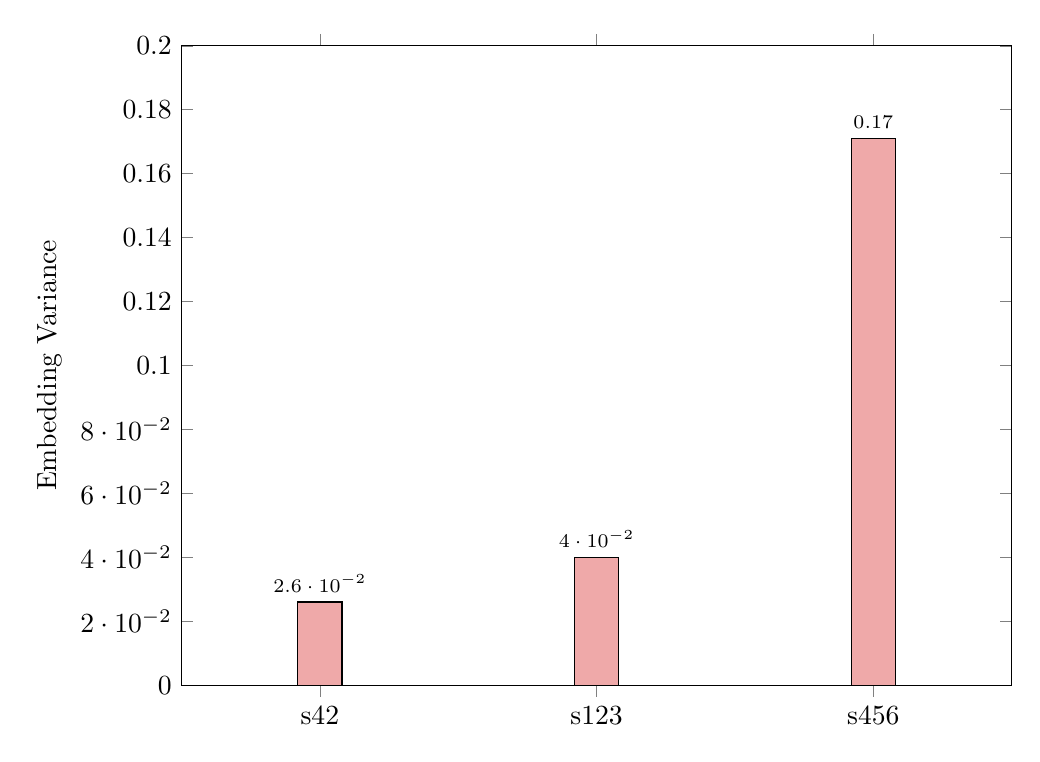
\begin{tikzpicture}
\begin{axis}[
    ybar, bar width=16pt, ylabel={Embedding Variance},
    symbolic x coords={s42,s123,s456}, xtick=data, ymin=0, ymax=0.20,
    width=\textwidth, height=0.8\textwidth, enlarge x limits=0.25,
    nodes near coords, every node near coord/.append style={font=\scriptsize},
]
\addplot[fill=capred!40, draw=black] coordinates {(s42,0.026) (s123,0.040) (s456,0.171)};
\end{axis}
\end{tikzpicture}
\caption{Embedding variance per seed.}
\end{subfigure}
\hfill
\begin{subfigure}[t]{0.48\textwidth}
\centering
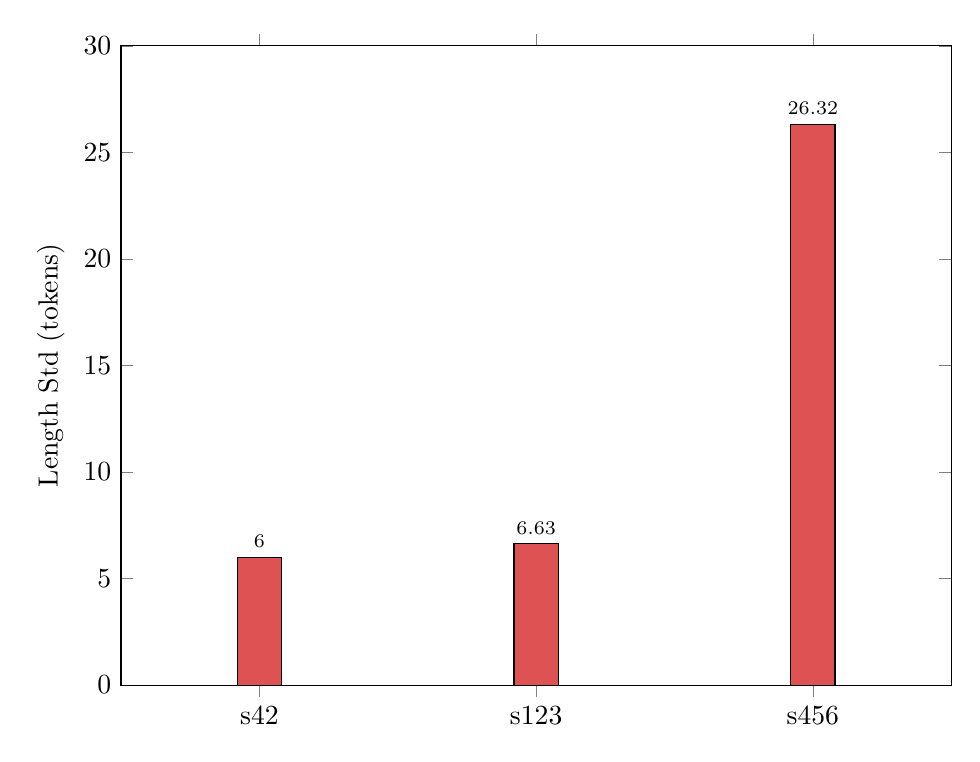
\begin{tikzpicture}
\begin{axis}[
    ybar, bar width=16pt, ylabel={Length Std (tokens)},
    symbolic x coords={s42,s123,s456}, xtick=data, ymin=0, ymax=30,
    width=\textwidth, height=0.8\textwidth, enlarge x limits=0.25,
    nodes near coords, every node near coord/.append style={font=\scriptsize},
]
\addplot[fill=capred!80, draw=black] coordinates {(s42,6) (s123,6.63) (s456,26.32)};
\end{axis}
\end{tikzpicture}
\caption{Length std per seed.}
\end{subfigure}
\caption{C6 per-seed bimodality: seeds 42, 123 internalize the cap; seed 456 does not.}
\label{fig:c6_bimodal}
\end{figure}

\subsection{Finding 3: KL Regularization Monotonically Increases Semantic Diversity}
\label{sec:finding3}

Embedding variance rises with $\beta$: $0.134 \rightarrow 0.134 \rightarrow 0.246 \rightarrow 0.286$ (baseline to $\beta=0.10$). An exact Jonckheere-Terpstra trend test across all 12 observations confirms this (one-sided $p=0.0009$; pass@1's decline gives $p=0.0005$). Pairwise, C1 vs.\ C5 gives $p=0.100$ (the $n=3$ floor) with Cohen's $d=-12.09$; C5 vs.\ C7 (Finding~\ref{find:c7combined}) gives $p=0.600$, $d=0.53$, consistent with near-equal means; C1 vs.\ C2 (Finding~\ref{find:hacking}) gives $p=0.600$, $d=-0.42$, consistent with seed noise. Full pairwise tests and bootstrap CIs are in Appendix~\ref{app:stats}.

C4 and C5 show tight seed agreement (SD at 9\% and 2\% of their means), the most seed-robust pattern in the study alongside C7 (Section~\ref{sec:c7}). C3 ($\beta=0.01$) is statistically indistinguishable from baseline in mean but carries near-half its own mean in SD, consistent with a below-threshold effect that depends on the seed.

\begin{finding}
\label{find:klmono}
KL regularization strength shows the most seed-robust relationship with semantic diversity we observe: embedding variance increases with $\beta$ from 0.05 upward, with tight cross-seed agreement at $\beta \geq 0.05$. We treat this as the paper's most confidently supported result.
\end{finding}

The cost is close to monotonic: pass@1 falls $0.21\pm0.04 \rightarrow 0.13\pm0.02 \rightarrow 0.13\pm0.03 \rightarrow 0.07\pm0.03$. Figure~\ref{fig:kl_tradeoff} visualizes this tradeoff.

\begin{figure}[t]
\centering
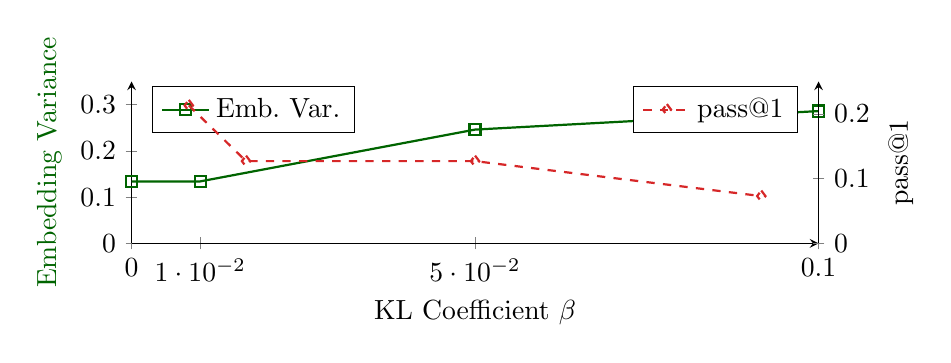
\begin{tikzpicture}
\begin{axis}[
    xlabel={KL Coefficient $\beta$}, ylabel={Embedding Variance},
    ylabel near ticks, ylabel style={color=klmedgreen},
    xtick={0, 0.01, 0.05, 0.10}, width=0.85\textwidth, height=0.3\textwidth,
    axis y line=left, axis x line=bottom, ymin=0, ymax=0.35, legend pos=north west,
]
\addplot[color=klmedgreen, mark=square, thick] coordinates {(0, 0.134) (0.01, 0.134) (0.05, 0.246) (0.10, 0.286)};
\addlegendentry{Emb.\ Var.}
\end{axis}
\begin{axis}[
    ylabel={pass@1}, ylabel near ticks, ylabel style={color=capred},
    xtick={0, 0.01, 0.05, 0.10}, width=0.85\textwidth, height=0.3\textwidth,
    axis y line=right, axis x line=none, ymin=0, ymax=0.25, legend pos=north east,
]
\addplot[color=capred, mark=diamond, thick, dashed] coordinates {(0, 0.213) (0.01, 0.127) (0.05, 0.127) (0.10, 0.073)};
\addlegendentry{pass@1}
\end{axis}
\end{tikzpicture}
\caption{KL exploration-exploitation tradeoff: embedding variance (left) rises, pass@1 (right) falls, with $\beta$. Means over 3 seeds.}
\label{fig:kl_tradeoff}
\end{figure}

\subsection{Finding 4 and Finding 5: The Two Diversity Metrics Disagree, and C7 Escapes the Resulting Tradeoff}
\label{sec:metricdivergence}

Table~\ref{tab:metric_corr} correlates our metrics (Section~\ref{sec:metrics}) across the seven condition means. Embedding variance and unique solution count are near-orthogonal ($r=-0.122$, $p=0.794$), while unique tracks pass@8 closely ($r=0.876$, $p=0.010$), the only pair reaching $p<0.05$ besides gap-unique. This is mechanistic: unique solution count only counts distinct \emph{correct} expressions, so it is bounded by how many completions are correct, exactly what pass@8 measures; embedding variance is computed over reasoning content regardless of correctness and has no such bound. This is why we treat embedding variance as primary and unique solution count as secondary and correctness-confounded (Section~\ref{sec:metrics}); this analysis is the evidence for that choice.

\begin{table}[h]
\centering
\caption{Pearson correlations across the seven condition means. Only two pairs reach $p<0.05$ at $n=7$.}
\label{tab:metric_corr}
\small
\begin{tabular}{lcc}
\toprule
\textbf{Metric pair} & \textbf{Pearson $r$} & \textbf{$p$} \\
\midrule
Emb.\ Var.\ vs.\ Unique & $-0.122$ & $0.794$ \\
Emb.\ Var.\ vs.\ pass@8 & $-0.402$ & $0.371$ \\
pass@8 vs.\ Unique & $0.876$ & $0.010$ \\
Gap vs.\ Unique & $0.778$ & $0.039$ \\
Gap vs.\ Emb.\ Var.\ & $0.120$ & $0.798$ \\
\bottomrule
\end{tabular}
\end{table}

Restricted to the four KL points, embedding variance and unique solution count move in nearly opposite directions ($0.134{\to}0.286$ vs.\ $0.49{\to}0.31$; $\beta$-embvar $r=0.963$, $\beta$-unique $r=-0.983$). Pairwise seed concordance (54 comparisons across the ordered groups) corroborates this informally: embedding variance increases in 88.9\% of pairs, unique decreases in 83.3\%.

\begin{finding}
\label{find:kltradeoff}
Within the KL sweep, embedding variance and unique solution count move in nearly opposite directions as $\beta$ increases (88.9\% and 83.3\% pairwise seed concordance). KL regularization does not simply increase diversity; it exchanges outcome diversity (how many different correct answers the policy finds) for process diversity (how varied its reasoning is regardless of outcome).
\end{finding}

At embedding variance statistically indistinguishable from C5 (C7: $0.282\pm0.010$ vs.\ C5: $0.286\pm0.007$, Mann-Whitney $p=0.507$), C7 achieves markedly higher unique solution count (0.453 vs.\ 0.313, $d=1.24$, $p=0.200$) and pass@8 (0.393 vs.\ 0.273, $d=2.30$, $p=0.100$). This is anchored specifically to C5: C7's unique solution count still ranks fourth of seven overall (behind C2, C3, C1), so the claim is that C7 escapes the tradeoff seen within the pure KL series at matched diversity, not that it leads the full table.

\begin{finding}
\label{find:c7escape}
At embedding variance statistically indistinguishable from the high-KL condition, the combined guardrail achieves markedly higher unique solution count and pass@8 than high-KL alone, while still ranking only fourth of seven overall on unique solution count.
\end{finding}

One plausible explanation is that C7's length cap prevents the unproductive length expansion seen in the pure-KL and hackable conditions (median length 78--140 tokens) from consuming the diversity that KL regularization enforces; bounded to $\sim$40 tokens, the same enforced diversity may manifest as variation across shorter, more often-correct paths instead. This is consistent with, though not established by, C7's shorter median length versus C5 (40.3 vs.\ 78.3, Section~\ref{sec:c7}). Figure~\ref{fig:metric_divergence} visualizes both findings.

\begin{figure}[t]
\centering
\begin{subfigure}[t]{0.48\textwidth}
\centering
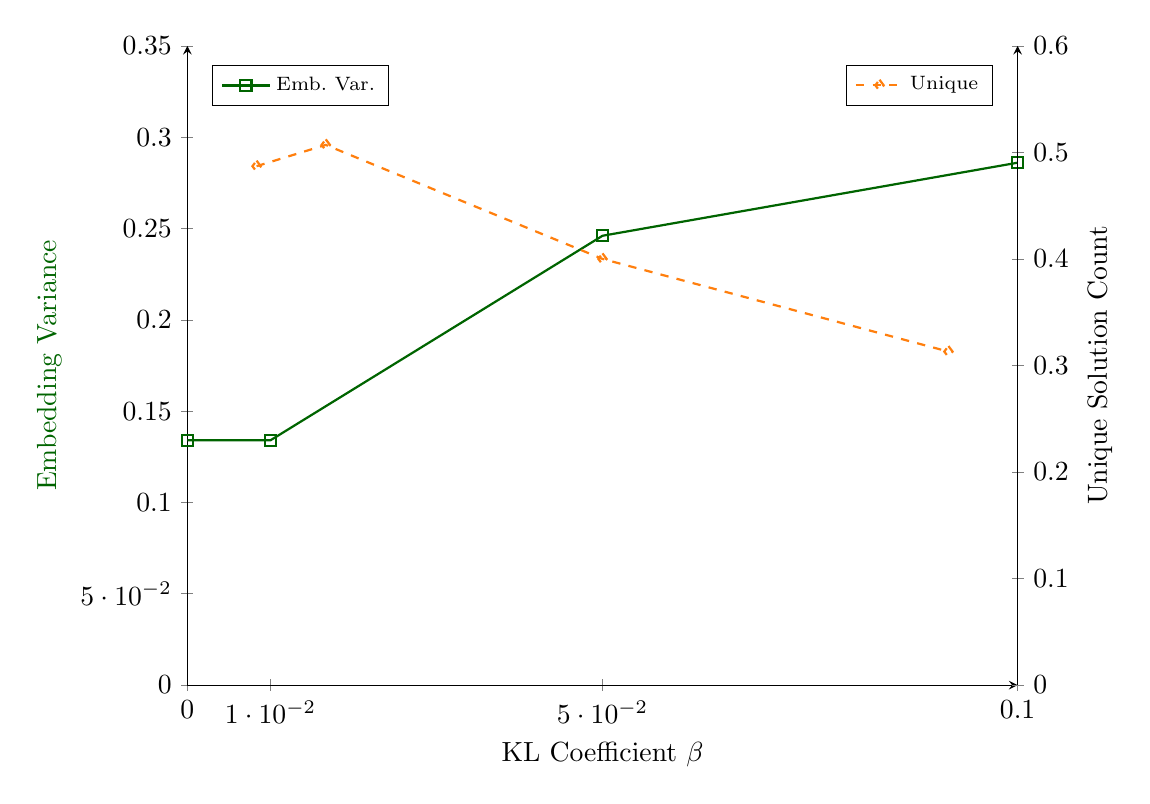
\begin{tikzpicture}
\begin{axis}[
    xlabel={KL Coefficient $\beta$}, ylabel={Embedding Variance},
    ylabel near ticks, ylabel style={color=klmedgreen},
    xtick={0, 0.01, 0.05, 0.10}, width=\textwidth, height=0.8\textwidth,
    axis y line=left, axis x line=bottom, ymin=0, ymax=0.35,
    legend pos=north west, legend style={font=\scriptsize},
]
\addplot[color=klmedgreen, mark=square, thick] coordinates {(0, 0.134) (0.01, 0.134) (0.05, 0.246) (0.10, 0.286)};
\addlegendentry{Emb.\ Var.}
\end{axis}
\begin{axis}[
    ylabel={Unique Solution Count}, ylabel near ticks, ylabel style={color=hackableorange},
    xtick={0, 0.01, 0.05, 0.10}, width=\textwidth, height=0.8\textwidth,
    axis y line=right, axis x line=none, ymin=0, ymax=0.6,
    legend pos=north east, legend style={font=\scriptsize},
]
\addplot[color=hackableorange, mark=diamond, thick, dashed] coordinates {(0, 0.487) (0.01, 0.507) (0.05, 0.400) (0.10, 0.313)};
\addlegendentry{Unique}
\end{axis}
\end{tikzpicture}
\caption{Embedding variance and unique count crossing as $\beta$ rises.}
\end{subfigure}
\hfill
\begin{subfigure}[t]{0.48\textwidth}
\centering
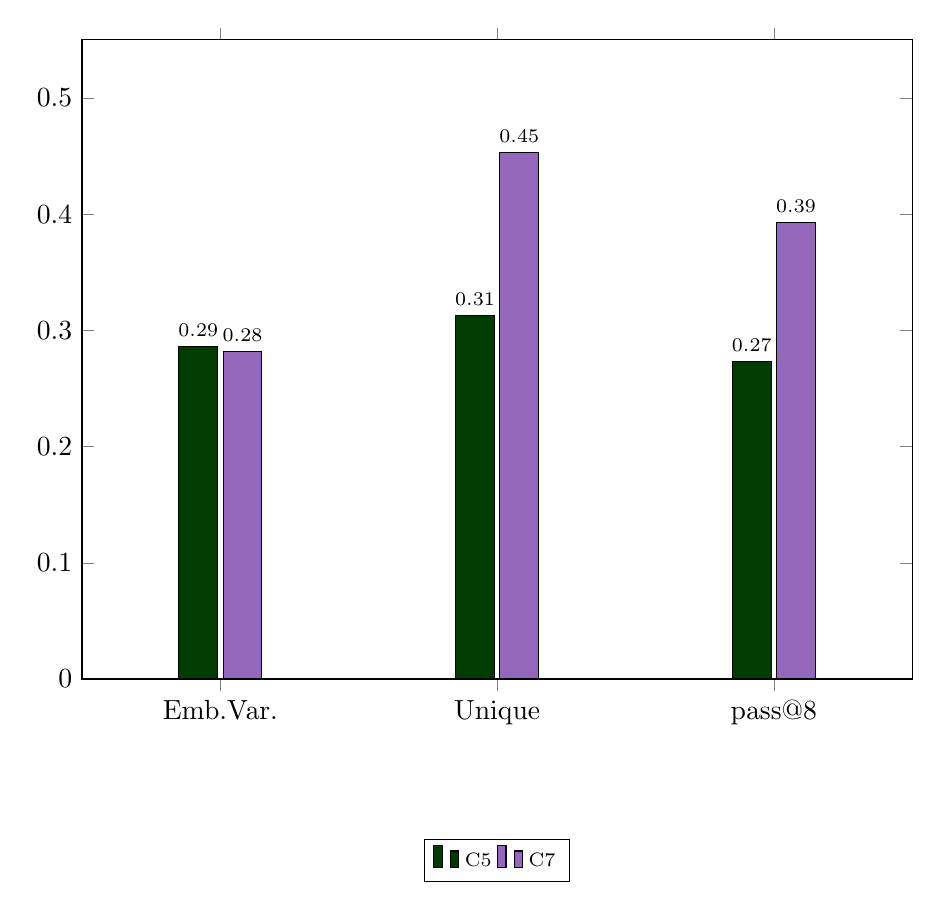
\begin{tikzpicture}
\begin{axis}[
    ybar, bar width=14pt, symbolic x coords={Emb.Var.,Unique,pass@8}, xtick=data,
    ymin=0, ymax=0.55, width=\textwidth, height=0.8\textwidth, enlarge x limits=0.25,
    nodes near coords, every node near coord/.append style={font=\scriptsize},
    legend style={at={(0.5,-0.25)}, anchor=north, legend columns=2, font=\scriptsize},
]
\addplot[fill=klhighgreen, draw=black] coordinates {(Emb.Var.,0.286) (Unique,0.313) (pass@8,0.273)};
\addlegendentry{C5}
\addplot[fill=comboguard, draw=black] coordinates {(Emb.Var.,0.282) (Unique,0.453) (pass@8,0.393)};
\addlegendentry{C7}
\end{axis}
\end{tikzpicture}
\caption{C5 vs.\ C7: matched embedding variance, C7 leads on the other two.}
\end{subfigure}
\caption{The KL tradeoff (Finding~\ref{find:kltradeoff}) and how C7 escapes it (Finding~\ref{find:c7escape}).}
\label{fig:metric_divergence}
\end{figure}

\subsection{Finding 6: Guardrail Mechanism, Not Reward Hacking, Determines Exploration}

Three conditions share the length bonus: no guardrail (C2, embvar 0.155), hard cap (C6, 0.079 average, bimodal per Section~\ref{sec:c6instability}), high KL (C5, 0.286). The cap suppresses hacking and, when internalized, collapses diversity; KL also suppresses hacking but consistently \emph{increases} diversity instead.

\begin{finding}
\label{find:guardrailmech}
Guardrail mechanism, not reward hacking itself, is the primary determinant of exploration behavior. A hard cap and a KL penalty move diversity in opposite directions from an identical reward function, and only the KL direction does so reliably across seeds.
\end{finding}

\subsection{Finding 7: Combining Guardrails Reproduces KL-Level Diversity at Lower Length, Reliably}
\label{sec:c7}

C7 combines $\beta=0.05$ with the 65-token cap. A single-seed pilot suggested C7 led on pass@8 and unique count; this did not replicate (three-seed pass@8 $0.39\pm0.06$, unique $0.45\pm0.14$, unremarkable). What did replicate is embedding variance: $0.282\pm0.010$ (SD 3.4\% of mean, one of the tightest results in the paper), matching C5 (0.286$\pm$0.007) at less than half the median length (40.3 vs.\ 78.3 tokens), with all three seeds in a narrow 0.273--0.292 band and 39--42 token median length (Appendix~\ref{app:supp}, Table~\ref{tab:c7_seeds}).

\begin{finding}
\label{find:c7combined}
Combining a hard length cap with moderate KL regularization reproduces the high semantic diversity of KL-only training at substantially shorter reasoning length, consistently across all three seeds, in contrast to the cap-alone condition's seed-dependent failure to internalize the constraint (Section~\ref{sec:c6instability}).
\end{finding}

This is about reliability and complementarity, not the correctness leaderboard: C7's pass@1 ($0.15\pm0.03$) is below baseline and roughly on par with C6's mean. Figure~\ref{fig:c7_comparison} (Appendix~\ref{app:supp}) compares C7 against C4 and C6 directly.

\subsection{Length Cap Severity Sweep}
\label{sec:sweep}

We additionally swept the cap threshold (45, 65, 100, 128 tokens) at a single seed (456), preliminary and not seed-replicated (full table and Spearman correlations in Appendix~\ref{app:supp}, Table~\ref{tab:sweep}). pass@1 is cleanly monotonic with cap size (0.06, 0.08, 0.10, 0.18); embedding variance is not, because the cap=65 point is the same non-internalizing seed-456 run from Section~\ref{sec:c6instability} (max length 216 against the cap). Excluding that documented outlier, embedding variance rises with cap size (0.015, 0.096, 0.102), consistent with tighter caps producing less diversity when the constraint is actually learned. The cap=45 run deserves separate mention: pass@1, pass@8, and unique count are all 0.06 with exploration gap exactly 0.00, so correctness is deterministic per problem, yet length SD is still 4.32 tokens (range 25--58), meaning surface wording still varies. This is a content and outcome collapse without a token-level repetition collapse, arguably a more severe failure mode than the cap=65 run's token explosion, and the cleanest illustration in the paper of a guardrail eliminating exploration outright.

\section{Discussion}

\textbf{Hard caps are effective but not dependable alone.} When internalized, a hard cap suppresses hacking and collapses exploration while preserving competitive pass@1; but internalization failed in one of three seeds, and in that seed the cap delivered neither its usual length control nor its diversity reduction. Practitioners should not assume a hard cap will behave identically every run.

\textbf{KL is the more seed-robust lever, but $\beta$ needs a minimum threshold.} At $\beta \geq 0.05$, diversity rises consistently across seeds at a monotonic accuracy cost; at $\beta=0.01$ the effect is inconsistent and indistinguishable from no regularization in mean.

\textbf{Combining a cap with moderate KL buys reliability, not correctness.} C7 reproduces high-KL diversity at much shorter length with tight cross-seed agreement the cap alone lacks, but does not outperform the individual guardrails on pass@1.

\textbf{Which diversity metric you report can flip the apparent verdict.} Scored by unique solution count, KL regularization looks purely costly, since unique count falls as $\beta$ rises (Section~\ref{sec:metricdivergence}); scored by embedding variance, the same runs look like they gain something valuable. For a verifier or guardrail meant to preserve exploration, this is not a minor detail: the same intervention can be judged a success or a failure depending on which diversity signal is checked, and we would encourage reporting both rather than the one that confirms the expected conclusion.

\textbf{The clean baseline still gives the best pass@1.} When hacking is mild, no guardrail gives the highest pass@1 ($0.21\pm0.04$) at diversity comparable to the guardrailed conditions' low end. Guardrails should not be applied reflexively.

\textbf{Limitations.} Small model scale (1.5B); a single, relatively simple task; 1000 training steps; three seeds for the core and combined conditions (adequate to separate a robust effect from a seed-dependent one, but limited for smaller effects, and we deliberately avoid significance tests at this $n$) versus one seed for the severity sweep; and a correlation analysis (Section~\ref{sec:metricdivergence}) computed over only seven condition means (or four KL points), which describes this specific design and should not be generalized to all GRPO settings. The unique solution count metric itself shows high seed variance in several conditions (e.g., C6: 0.06, 0.40, 0.36) independent of the cap-internalization failure, reinforcing embedding variance as the more dependable primary metric. Full discussion in Appendix~\ref{app:stats}.

\textbf{Broader impact.} This is foundational empirical work on RL training dynamics for a small open model on a synthetic arithmetic task; we see no direct dual-use or deployment risk. The main practical risk we would flag is the inverse of a typical broader-impact concern: a practitioner who assumes a guardrail (especially a hard cap) reliably reduces or preserves diversity, based on a single training run, may be wrong roughly one seed in three in our data, which matters if diversity-preserving guardrails are deployed as a safety or fairness measure rather than validated across seeds.

\section{Conclusion}

Guardrail mechanism, not reward hacking itself, determines exploration behavior in our GRPO setting, and how reliably it does so depends on the mechanism. KL regularization gives a diverse but less accurate policy, consistently once $\beta$ clears a minimum threshold. A hard cap gives either a narrow, repetitive policy or, one seed in three here, a policy that never internalizes the constraint. Combining both reproduces most of KL's diversity benefit at a fraction of the length. Reward hacking alone leaves diversity within baseline noise. Most consequentially for verifier design, our two diversity metrics disagree with each other in a mechanistically explicable way, so the choice of diversity metric, not only the choice of guardrail, shapes the apparent conclusion. Guardrail design is an implicit exploration-exploitation decision, but not always a reliable one, and evaluating it on a single metric or a single seed can be actively misleading. Future work should extend to larger models, more diverse tasks, and enough seeds to characterize failure rates (of cap internalization, and of metric agreement) rather than observe them once.

\begin{ack}
This work received no external funding, and the author declares no competing interests.
\end{ack}

\bibliographystyle{unsrt}
\bibliography{references}

\appendix

\section{Raw Per-Seed Results}
\label{app:raw_data}

\begin{table}[h]
\centering
\caption{Raw per-seed evaluation results, six core conditions and C7, three seeds each.}
\label{tab:raw}
\small
\begin{tabular}{lcccccc}
\toprule
\textbf{Condition - Seed} & \textbf{pass@1} & \textbf{pass@8} & \textbf{Gap} & \textbf{Unique} & \textbf{Emb. Var.} & \textbf{Med. Len.} \\
\midrule
C1-42  & 0.20 & 0.48 & 0.28 & 0.58 & 0.153 & 38.0 \\
C1-123 & 0.26 & 0.40 & 0.14 & 0.50 & 0.123 & 34.0 \\
C1-456 & 0.18 & 0.32 & 0.14 & 0.38 & 0.126 & 44.0 \\
\midrule
C2-42  & 0.14 & 0.38 & 0.24 & 0.46 & 0.205 & 130.5 \\
C2-123 & 0.16 & 0.46 & 0.30 & 0.68 & 0.077 & 138.0 \\
C2-456 & 0.16 & 0.44 & 0.28 & 0.60 & 0.182 & 135.0 \\
\midrule
C3-42  & 0.10 & 0.46 & 0.36 & 0.58 & 0.079 & 159.0 \\
C3-123 & 0.14 & 0.36 & 0.22 & 0.48 & 0.200 & 115.0 \\
C3-456 & 0.14 & 0.34 & 0.20 & 0.46 & 0.122 & 145.0 \\
\midrule
C4-42  & 0.16 & 0.34 & 0.18 & 0.42 & 0.221 & 112.0 \\
C4-123 & 0.10 & 0.28 & 0.18 & 0.36 & 0.251 & 113.0 \\
C4-456 & 0.12 & 0.34 & 0.22 & 0.42 & 0.265 & 98.5 \\
\midrule
C5-42  & 0.08 & 0.26 & 0.18 & 0.26 & 0.293 & 83.5 \\
C5-123 & 0.04 & 0.24 & 0.20 & 0.28 & 0.280 & 90.0 \\
C5-456 & 0.10 & 0.32 & 0.22 & 0.40 & 0.285 & 61.5 \\
\midrule
C6-42  & 0.22 & 0.38 & 0.16 & 0.06 & 0.026 & 64.0 \\
C6-123 & 0.16 & 0.30 & 0.14 & 0.40 & 0.040 & 61.0 \\
C6-456 & 0.08 & 0.30 & 0.22 & 0.36 & 0.171 & 52.0 \\
\midrule
C7-42  & 0.14 & 0.38 & 0.24 & 0.44 & 0.292 & 39.0 \\
C7-123 & 0.18 & 0.34 & 0.16 & 0.32 & 0.273 & 42.0 \\
C7-456 & 0.12 & 0.46 & 0.34 & 0.60 & 0.280 & 40.0 \\
\bottomrule
\end{tabular}
\end{table}

\section{Statistical Analysis}
\label{app:stats}

Given $n=3$ seeds per condition, all tests are exact and non-parametric; we do not report $p$-values from parametric tests anywhere in this paper.

\begin{table}[h]
\centering
\caption{BCa bootstrap 95\% CIs for embedding variance and pass@1, 3 seeds, 10,000 resamples. At $n=3$ these are rough uncertainty sketches, not precise inferential bounds; corroborate with the permutation tests in Section~\ref{sec:finding3} before reading overlap or separation as significance.}
\label{tab:bootstrap_ci}
\small
\begin{tabular}{lcccc}
\toprule
\textbf{Condition} & \textbf{Mean Emb.\ Var.} & \textbf{95\% BCa CI} & \textbf{Mean pass@1} & \textbf{95\% BCa CI} \\
\midrule
C1: Baseline  & 0.134 & [0.123, 0.144] & 0.213 & [0.180, 0.240] \\
C2: Hackable  & 0.155 & [0.077, 0.197] & 0.153 & [0.140, 0.160] \\
C3: KL-Low    & 0.134 & [0.079, 0.174] & 0.127 & [0.100, 0.140] \\
C4: KL-Med    & 0.246 & [0.221, 0.260] & 0.127 & [0.100, 0.147] \\
C5: KL-High   & 0.286 & [0.280, 0.290] & 0.073 & [0.040, 0.093] \\
C6: LengthCap & 0.079 & [0.026, 0.127] & 0.153 & [0.080, 0.220] \\
C7: Combined  & 0.282 & [0.273, 0.288] & 0.147 & [0.120, 0.167] \\
\bottomrule
\end{tabular}
\end{table}

\begin{table}[h]
\centering
\caption{Coefficient of variation (CV = SD/mean) for embedding variance across 3 seeds, most to least seed-robust. C6 is least reliable (CV $>1$), driven by seed 456's cap-internalization failure.}
\label{tab:cv_ranking}
\small
\begin{tabular}{clccc}
\toprule
\textbf{Rank} & \textbf{Condition} & \textbf{Mean Emb.\ Var.} & \textbf{SD} & \textbf{CV} \\
\midrule
1 & C5: KL-High  & 0.286 & 0.007 & 0.023 \\
2 & C7: Combined & 0.282 & 0.010 & 0.034 \\
3 & C4: KL-Med   & 0.246 & 0.022 & 0.092 \\
4 & C1: Baseline & 0.134 & 0.017 & 0.123 \\
5 & C2: Hackable & 0.155 & 0.068 & 0.441 \\
6 & C3: KL-Low   & 0.134 & 0.061 & 0.459 \\
7 & C6: LengthCap& 0.079 & 0.080 & 1.012 \\
\bottomrule
\end{tabular}
\end{table}

At $n=3$ per group, exact permutation tests over all relabelings achieve a minimum two-sided $p$ of 0.10 ($\binom{6}{3}=20$ relabelings); no result can register as conventionally significant regardless of effect size, and $p$ in 0.10--0.30 should read as ``suggestive but not conclusive,'' not ``non-significant.'' BCa intervals above are similarly unstable at $n=3$, since both the resampling distribution and the jackknife acceleration term derive from only three points; treat them as rough uncertainty sketches, and do not read CI overlap or separation alone as a significance statement. The C6 severity sweep (Appendix~\ref{app:supp}) is single-seed with no replication, precluding any claim that a cap value's behavior is a property of the cap rather than of that seed's trajectory; its Spearman correlations are descriptive of one run per cap, and the post hoc exclusion of the cap=65 outlier is exploratory, not confirmatory. Readers should conclude, at most, that the effect sizes and rank orderings reported throughout this paper are directionally consistent with our qualitative claims, not that any specific pairwise difference or trend has been statistically established at this sample size.

\section{Supplementary Tables, Figures, and Qualitative Examples}
\label{app:supp}

\begin{table}[h]
\centering
\caption{C7 per-seed breakdown. Embedding variance and median length are tightly clustered across all three seeds, contrast with C6 (Table~\ref{tab:c6_seeds}).}
\label{tab:c7_seeds}
\small
\begin{tabular}{lccccc}
\toprule
\textbf{Seed} & \textbf{pass@1} & \textbf{pass@8} & \textbf{Unique} & \textbf{Emb.\ Var.} & \textbf{Med.\ Len.} \\
\midrule
42  & 0.14 & 0.38 & 0.44 & 0.292 & 39.0 \\
123 & 0.18 & 0.34 & 0.32 & 0.273 & 42.0 \\
456 & 0.12 & 0.46 & 0.60 & 0.280 & 40.0 \\
\bottomrule
\end{tabular}
\end{table}

\begin{figure}[h]
\centering
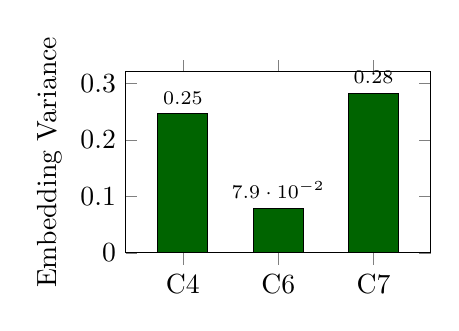
\begin{tikzpicture}
\begin{axis}[
    ybar, bar width=18pt, ylabel={Embedding Variance}, symbolic x coords={C4,C6,C7},
    xtick=data, ymin=0, ymax=0.32, width=0.45\textwidth, height=0.32\textwidth,
    enlarge x limits=0.3, nodes near coords, every node near coord/.append style={font=\scriptsize},
]
\addplot[fill=klmedgreen, draw=black] coordinates {(C4,0.246) (C6,0.079) (C7,0.282)};
\end{axis}
\end{tikzpicture}
\hfill
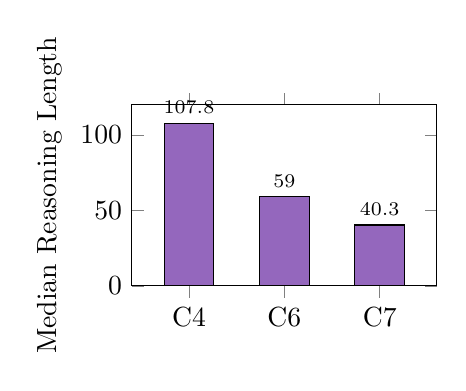
\begin{tikzpicture}
\begin{axis}[
    ybar, bar width=18pt, ylabel={Median Reasoning Length}, symbolic x coords={C4,C6,C7},
    xtick=data, ymin=0, ymax=120, width=0.45\textwidth, height=0.32\textwidth,
    enlarge x limits=0.3, nodes near coords, every node near coord/.append style={font=\scriptsize},
]
\addplot[fill=comboguard, draw=black] coordinates {(C4,107.8) (C6,59.0) (C7,40.3)};
\end{axis}
\end{tikzpicture}
\caption{C7 alongside C4 (KL alone) and C6 (cap alone). C7 reaches C4-or-higher embedding variance at a fraction of C4's length, more reliably than C6. C6's bar is the raw three-seed mean; see Table~\ref{tab:c6_seeds} for per-seed values.}
\label{fig:c7_comparison}
\end{figure}

\begin{table}[h]
\centering
\caption{Length cap severity sweep, single seed (456), preliminary. The cap-65 row is the seed-456 C6 run (Section~\ref{sec:c6instability}) that failed to internalize the constraint; kept here rather than removed. Spearman $\rho$ (cap size vs.\ metric, all 4 points / excluding cap=65): pass@1 $1.00/1.00$, Emb.\ Var.\ $0.40/1.00$, Med.\ Len.\ $1.00/1.00$, Len.\ Std $0.80/0.50$.}
\label{tab:sweep}
\small
\begin{tabular}{lcccccccc}
\toprule
\textbf{Cap} & \textbf{pass@1} & \textbf{pass@8} & \textbf{Gap} & \textbf{Unique} & \textbf{Emb.\ Var.} & \textbf{Med.\ Len.} & \textbf{Len.\ Std} & \textbf{Min/Max} \\
\midrule
45  & 0.06 & 0.06 & 0.00 & 0.06 & 0.015 & 44.0 & 4.32 & 25/58 \\
65$^*$ & 0.08 & 0.30 & 0.22 & 0.36 & 0.171 & 52.0 & 26.32 & 0/216 \\
100 & 0.10 & 0.26 & 0.16 & 0.28 & 0.096 & 92.0 & 37.20 & 0/250 \\
128 & 0.18 & 0.36 & 0.18 & 0.48 & 0.102 & 96.0 & 30.81 & 0/245 \\
\bottomrule
\end{tabular}
\end{table}

\textbf{Training dynamics.} Figures available from the original seed-42/123 W\&B runs (not reproduced here for space) show C2 and C3 think-length increasing gradually over training rather than being present from initialization; C6 think length is flat and bounded for these two seeds, consistent with Table~\ref{tab:c6_seeds}, and predates the non-internalizing seed-456 run shown directly in Figure~\ref{fig:c6_bimodal}. C3 shows early correctness spikes followed by degradation, consistent with the below-threshold instability in Finding~\ref{find:klmono}.

\textbf{Qualitative example.} For the prompt with numbers $[5, 96, 84, 1]$, target 75: a C2 (hackable) completion reasons ``Start with 96 and subtract 1 to get 95. Add 84 to 95 to get 189. Subtract 5 from 189 to get 184. The number 1 is not needed, so remove it. Thus, 96 - 1 + 84 - 5,'' long, meandering, and internally inconsistent (the stated intermediate value 184 does not match the final expression's evaluation). A C6 (length cap, internalizing seed) completion for the same prompt reasons ``combine these numbers in a way that results in 75'' before giving \texttt{(84 - 96) + 1}, shorter and, consistent with Finding~\ref{find:c6bimodal} for an internalizing seed, semantically repetitive across samples.

\newpage
\section*{NeurIPS Paper Checklist}

\begin{enumerate}

\item {\bf Claims}
    \item[] Question: Do the main claims made in the abstract and introduction accurately reflect the paper's contributions and scope?
    \item[] Answer: \answerYes{}
    \item[] Justification: The abstract and introduction state each finding scoped exactly to the statistical evidence behind it (seed counts, effect sizes, the $n=3$ exact-test $p$-floor), including the two findings that were revised downward relative to an earlier single-seed pilot (the hard-cap collapse and the C7 leaderboard claim); see Sections 4 and Appendix B for the underlying tests.

\item {\bf Limitations}
    \item[] Question: Does the paper discuss the limitations of the work performed by the authors?
    \item[] Answer: \answerYes{}
    \item[] Justification: The Discussion's Limitations paragraph (Section 5) covers model scale, single-task scope, training duration, seed count and statistical power, the single-seed status of the cap severity sweep, the descriptive-only scope of the metric-correlation analysis, and unique solution count's own seed variance; a separate Broader Impact paragraph discusses the risk of over-trusting a guardrail validated on one seed.

\item {\bf Theory assumptions and proofs}
    \item[] Question: For each theoretical result, does the paper provide the full set of assumptions and a complete (and correct) proof?
    \item[] Answer: \answerNA{}
    \item[] Justification: This is a purely empirical study; the paper contains no theorems, lemmas, or formal proofs.

\item {\bf Experimental result reproducibility}
    \item[] Question: Does the paper fully disclose all the information needed to reproduce the main experimental results of the paper to the extent that it affects the main claims and/or conclusions of the paper (regardless of whether the code and data are provided or not)?
    \item[] Answer: \answerYes{}
    \item[] Justification: Section 3 specifies the base model, LoRA configuration (rank, alpha, dropout, target layers), all GRPO training hyperparameters, the public dataset and evaluation holdout protocol, all seven conditions' reward components (Table 1), the three training seeds, and the GPU used.

\item {\bf Open access to data and code}
    \item[] Question: Does the paper provide open access to the data and code, with sufficient instructions to faithfully reproduce the main experimental results, as described in supplemental material?
    \item[] Answer: \answerNo{}
    \item[] Justification: Code and trained checkpoints are not yet publicly released at submission time. The dataset used is a public HuggingFace dataset (\texttt{Jiayi-Pan/Countdown-Tasks-3to4}), and the full training/evaluation configuration needed to reimplement the pipeline is described in Section 3 and Table 1.

\item {\bf Experimental setting/details}
    \item[] Question: Does the paper specify all the training and test details (e.g., data splits, hyperparameters, how they were chosen, type of optimizer) necessary to understand the results?
    \item[] Answer: \answerYes{}
    \item[] Justification: Section 3 reports the model, LoRA hyperparameters, training steps, batch size, gradient accumulation, learning rate and schedule, GRPO group size, the fixed evaluation holdout (independent of training seed), and per-condition reward configuration in Table 1.

\item {\bf Experiment statistical significance}
    \item[] Question: Does the paper report error bars suitably and correctly defined or other appropriate information about the statistical significance of the experiments?
    \item[] Answer: \answerYes{}
    \item[] Justification: Section 3 (``Seeds and statistics'') and Appendix B state the factor of variability (training seed, $n=3$), the exact non-parametric tests used (Jonckheere-Terpstra, exact permutation, Mann-Whitney), Cohen's $d$ effect sizes reported alongside every $p$-value, and BCa bootstrap 95\% confidence intervals (Appendix B, Table~\ref{tab:bootstrap_ci}), with an explicit statement that the minimum achievable two-sided $p$ at $n=3$ is 0.10 so readers do not over-interpret $p$-values as conventional significance.

\item {\bf Experiments compute resources}
    \item[] Question: For each experiment, does the paper provide sufficient information on the computer resources (type of compute workers, memory, time of execution) needed to reproduce the experiments?
    \item[] Answer: \answerNo{}
    \item[] Justification: Section 3 reports the GPU type used (a single NVIDIA A10G per condition-seed run) but does not report exact wall-clock time or aggregate GPU-hours across the full study.

\item {\bf Code of ethics}
    \item[] Question: Does the research conducted in the paper conform, in every respect, with the NeurIPS Code of Ethics \url{https://neurips.cc/public/EthicsGuidelines}?
    \item[] Answer: \answerYes{}
    \item[] Justification: The work fine-tunes an open-weight language model on a public synthetic arithmetic dataset with no human subjects, personal data, or dual-use application, and raises no departures from the Code of Ethics.

\item {\bf Broader impacts}
    \item[] Question: Does the paper discuss both potential positive societal impacts and negative societal impacts of the work performed?
    \item[] Answer: \answerYes{}
    \item[] Justification: The Broader Impact paragraph in the Discussion notes this is foundational RL-training-dynamics research with no direct deployment or dual-use risk, and flags the specific practical risk that a practitioner treating a guardrail's diversity effect as reliable from a single training run can be wrong roughly one seed in three in our data.

\item {\bf Safeguards}
    \item[] Question: Does the paper describe safeguards that have been put in place for responsible release of data or models that have a high risk for misuse (e.g., pre-trained language models, image generators, or scraped datasets)?
    \item[] Answer: \answerNA{}
    \item[] Justification: No models, datasets, or other assets with a high risk of misuse are released as part of this work.

\item {\bf Licenses for existing assets}
    \item[] Question: Are the creators or original owners of assets (e.g., code, data, models), used in the paper, properly credited and are the license and terms of use explicitly mentioned and properly respected?
    \item[] Answer: \answerNo{}
    \item[] Justification: The base model (Qwen2.5-1.5B-Instruct) and the Countdown dataset (\texttt{Jiayi-Pan/Countdown-Tasks-3to4} on HuggingFace) are both cited with source in Section 3 and the references, but their specific license terms are not individually restated in the paper text.

\item {\bf New assets}
    \item[] Question: Are new assets introduced in the paper well documented and is the documentation provided alongside the assets?
    \item[] Answer: \answerNA{}
    \item[] Justification: The paper does not release a new dataset or model as a packaged, documented asset; the trained LoRA adapters produced during the study are experimental artifacts, not a contribution of the paper.

\item {\bf Crowdsourcing and research with human subjects}
    \item[] Question: For crowdsourcing experiments and research with human subjects, does the paper include the full text of instructions given to participants and screenshots, if applicable, as well as details about compensation (if any)?
    \item[] Answer: \answerNA{}
    \item[] Justification: The paper does not involve crowdsourcing or research with human subjects.

\item {\bf Institutional review board (IRB) approvals or equivalent for research with human subjects}
    \item[] Question: Does the paper describe potential risks incurred by study participants, whether such risks were disclosed to the subjects, and whether Institutional Review Board (IRB) approvals (or an equivalent approval/review based on the requirements of your country or institution) were obtained?
    \item[] Answer: \answerNA{}
    \item[] Justification: The paper does not involve human subjects research.

\item {\bf Declaration of LLM usage}
    \item[] Question: Does the paper describe the usage of LLMs if it is an important, original, or non-standard component of the core methods in this research? Note that if the LLM is used only for writing, editing, or formatting purposes and does \emph{not} impact the core methodology, scientific rigor, or originality of the research, declaration is not required.
    \item[] Answer: \answerYes{}
    \item[] Justification: An LLM-based coding assistant was used beyond writing and formatting: it was used to debug the training/evaluation codebase, to compute and independently cross-check the statistical results reported in Section 4 and Appendix B (correlations, Cohen's $d$, exact permutation and Mann-Whitney tests, BCa bootstrap intervals) against the underlying per-seed logs, and to draft manuscript text. The experimental design, GRPO training runs, and evaluation data collection were carried out by the author's own training pipeline, independent of the LLM. \textbf{[Author: please review and adjust this justification to accurately reflect your own process before submission; this is a first-person disclosure I cannot finalize on your behalf.]}

\end{enumerate}


\end{document}
